\title{Parallax}
\author{
  Luke Hodkinson \\
  Center for Astrophysics and Supercomputing \\
  Swinburne University of Technology \\
  Melbourne, Hawthorn 32000, \underline{Australia}
}
\date{\today}

\documentclass[12pt]{scrartcl}
\usepackage{color}
\usepackage[usenames,dvipsnames]{xcolor}
\usepackage{amsmath}
\usepackage{amsfonts}
\usepackage{amssymb}
\usepackage{siunitx}
\usepackage{listings}
\usepackage{hyperref}
%% \usepackage[scaled]{beramono}
%% \renewcommand*\familydefault{\ttdefault}
%% \usepackage[Tl]{fontenc}

% Setup the tikz package for pictures.
\usepackage{tikz}
\usetikzlibrary{calc}
\usetikzlibrary{arrows}
\usetikzlibrary{shapes,decorations.pathmorphing}

\newcommand{\deriv}[2]{\ensuremath{\frac{\mathrm{d}#1}{\mathrm{d}#2}}}
\newcommand{\sderiv}[2]{\ensuremath{\frac{\mathrm{d}^2#1}{\mathrm{d}#2^2}}}
\newcommand{\dx}[1]{\ensuremath{\,\mathrm{d}#1}}

%% \lstset{
%%   language=Python,
%%   showstringspaces=false,
%%   formfeed=\newpage,
%%   tabsize=4,
%%   basicstyle=\small\ttfamily,
%%   commentstyle=\color{BrickRed}\itshape,
%%   keywordstyle=\color{blue},
%%   stringstyle=\color{OliveGreen},
%%   morekeywords={models, lambda, forms, dict, list, str, import, dir, help,
%%    zip, with, open}
%% }

\begin{document}
\maketitle

\section{The Observer's Triangle}

The part where they are equating $\sin \theta$ to $\theta$ is a result of the
Observer's Triangle. This typically only holds for triangles which subtend an angle of
less than 1 degree (that produces an error of less than 1\%). It works by realising
that the shorter edge of a long skinny triangle can be approximated
quite well as the length of the arc of the circle that triangle makes, where the
radius of the circle is the hypotenuse of the triangle (figure ~\ref{fig:observer}).
\begin{figure}[h]
\centering
  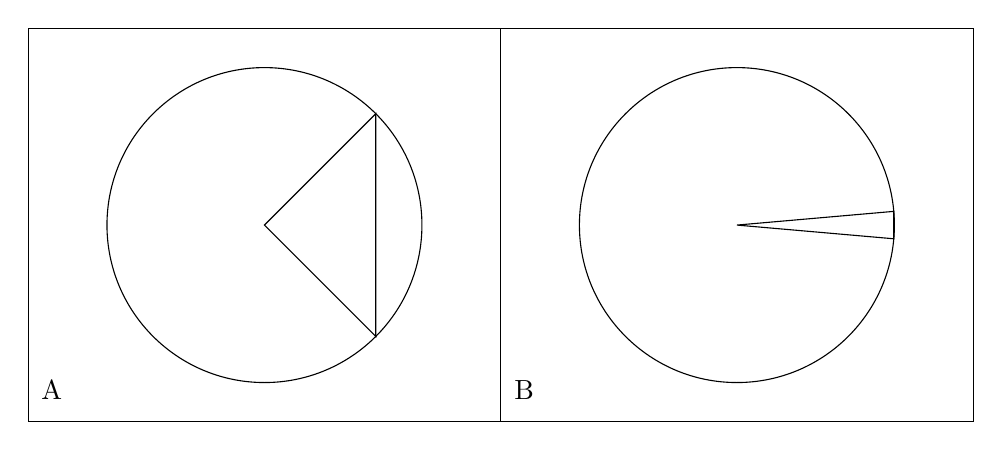
\begin{tikzpicture}
    \draw (0,0) rectangle(12,5);
    \draw (6,0) -- (6,5);
    \draw (3,2.5) circle(2);
    \draw (3,2.5) -- (4.414,3.914) -- (4.414,1.086) -- cycle;
    \draw (9,2.5) circle(2);
    \draw (9,2.5) -- (10.992,2.674) -- (10.992,2.326) -- cycle;
    \node at (0.3,0.4) {A};
    \node at (6.3,0.4) {B};
  \end{tikzpicture}
\caption{The Observer's triangle. In part A the angle of the triangle is large enough
that the edge opposite the angle is considerably shorter than the arc the triangle
makes with the circle. In part B those two quantities are effectively the same (actually
the angle should be a bit smaller, but it's still illustrative).}
\label{fig:observer}
\end{figure}
Now, using a little ratio logic we can relate the angle to the arc it subtends. Operating
in radians we know that there are $2\pi$ radians in a circle, and also there the
entire circumference of a circle is $2\pi r$, where $r$ is the radius of the circle. We
know that ratio of the angle to the total number of radians in a circle must be equal
to the ratio of the length of the arc subtended to the total circumference,
\begin{eqnarray*}
\frac{\theta}{2\pi} &=& \frac{l}{2\pi r} \\
\theta &=& \frac{l}{r} \; ,
\end{eqnarray*}
where $l$ is the length of the arc subtended (figure ~\ref{fig:ratio}).
\begin{figure}[h]
\centering
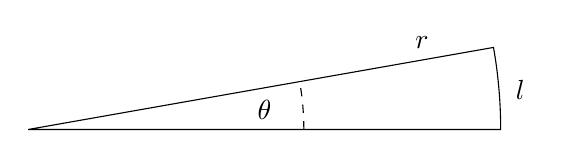
\begin{tikzpicture}
  \draw (0,0) -- (6,0) arc (0:10:6) -- (0,0);
  \draw[dashed] (3.5,0) arc (0:10:3.5);
  \node at (3,0.25) {$\theta$};
  \node at (6.25,0.5) {$l$};
  \node at (5,1.1) {$r$};
\end{tikzpicture}
\caption{Diagram relating arc length, radius and angle.}
\label{fig:ratio}
\end{figure}

Now, this is where we can equate $\sin \theta$ and $\theta$. From good old fashioned
trigonometry we know that
\[ \sin \theta = \frac{d}{r} \;, \]
where $d$ is the edge length opposite the angle. In our Observer's Triangle approximation
we've said that the opposite edge and the arc length are considered the same ($d \approx l$),
giving us:
\begin{eqnarray*}
\sin \theta &=& \frac{d}{r} \\
&\approx& \frac{l}{r} \\
&=& \theta \; ,
\end{eqnarray*}
therefore
\[ \sin \theta \approx \theta\]
under the Overver's Triangle assumption.

There are actually other ways to show the identity that $\sin \theta \approx \theta$ for
small angles, but this way is directly related to the problem we're trying to solve
(that being finding the distance to something). In addition, the following identites
are also true for small angled triangles:
\begin{eqnarray*}
\tan \theta &\approx& \theta \\
\cos \theta &\approx& 1 - \frac{\theta^2}{2}
\end{eqnarray*}

\end{document}
